\documentclass{article}

\usepackage{amsmath}
\usepackage{wrapfig}
\usepackage{amssymb}
\usepackage{graphicx}
\usepackage{biblatex}
\usepackage{listings}
\usepackage{xcolor}

\definecolor{backcolour}{rgb}{0.95,0.95,0.92}

\lstdefinestyle{mystyle}{
    backgroundcolor=\color{backcolour},
    basicstyle=\ttfamily\footnotesize,
    breakatwhitespace=false,
    breaklines=true,
    captionpos=b,
    keepspaces=true,
    showspaces=false,
    showstringspaces=false,
    showtabs=false,
    tabsize=2
}

\lstset{style=mystyle}

\begin{document}

  \section{Figures}
  
  \subsection{Figures with and without captions}
  
  This document is meant to exemplify the use of figures.
  
  \graphicspath{{tests/images/}}
  
  \begin{figure}[h]
  
    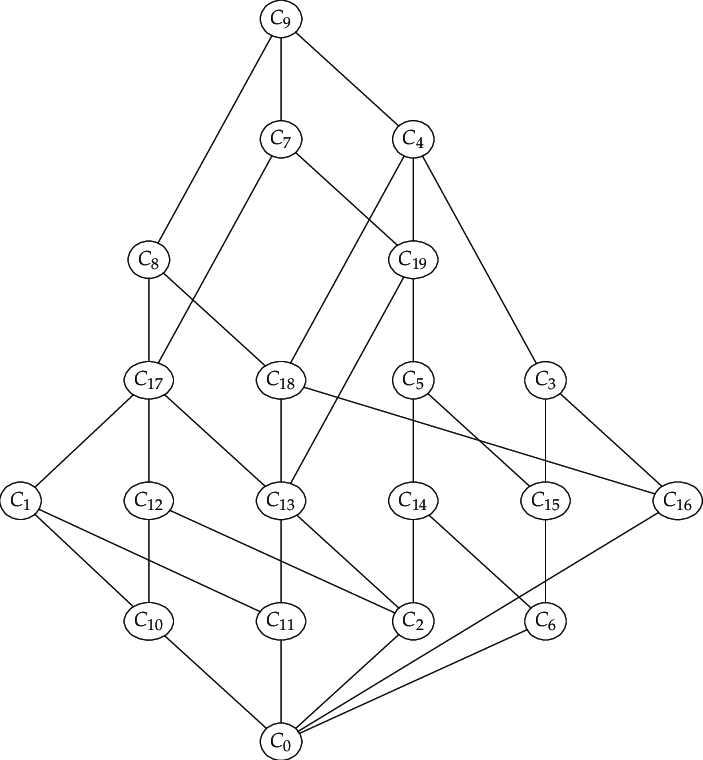
\includegraphics{complete_lattice}
  
  \end{figure}
  
  \begin{figure}[h]
  
    \caption{Now with a caption}
    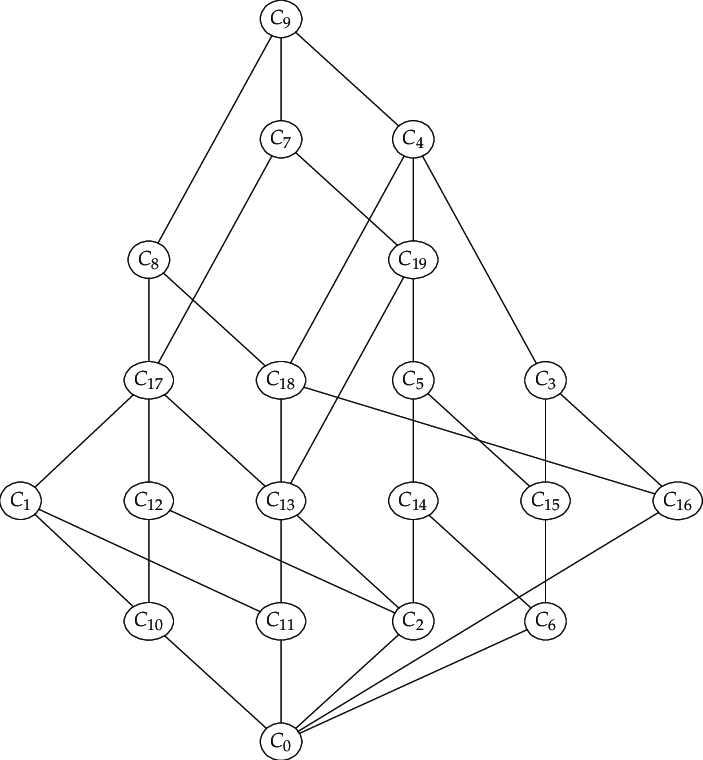
\includegraphics{complete_lattice}
  
  \end{figure}
  
  Amazing, isn't it?

\end{document} 

